
Para poder realizar las simulaciones en \cw\ se ha trabajado con una corriente de inyección constante e igual a la corriente de polarización ($I(t) = I_{Bias}$), tomando $V_{RF} = 0$.

HABLAR DE QUE EN CONTINUA SE TIENE QUE $\frac{\mathrm{d} N}{\mathrm{d} t} = \frac{\mathrm{d} S}{\mathrm{d} t} = \frac{\mathrm{d} \Phi}{\mathrm{d} t} = 0$

\addtocontents{toc}{\vspace{0.1cm}}
\subsection{Espectros de emisión}

	Tal y como se vio en la secci\'on \ref{Intr:LsrSmcdtr}, pequeñas variaciones en la corriente de inyección del láser producen desplazamientos de la línea de emisión del láser en el espectro de frecuencias. Por ello es importante conocer el valor de la longitud de onda del pico de emisión del láser en solitario en función de la corriente de polarización \ibias, de cara a realizar el estudio de la inyección de luz.

	En la Figura \ref{Img:spectrosCW} se muestran las densidades espectrales de potencia del l\'aser a diferentes corrientes de polarización, comparando los datos obtenidos mediante la simulaci\'on del l\'aser(Figura \ref{Img:spectrosCW:sim}), con los obtenidos experimentalmente(Figura \ref{Img:spectrosCW:exp}).

		% Img:spectrosCW {Img:spectrosCW:sim, Img:spectrosCW:exp}
		\begin{figure}[H]
			\centering
			\begin{subfigure}{0.45\textwidth}
				\centering
				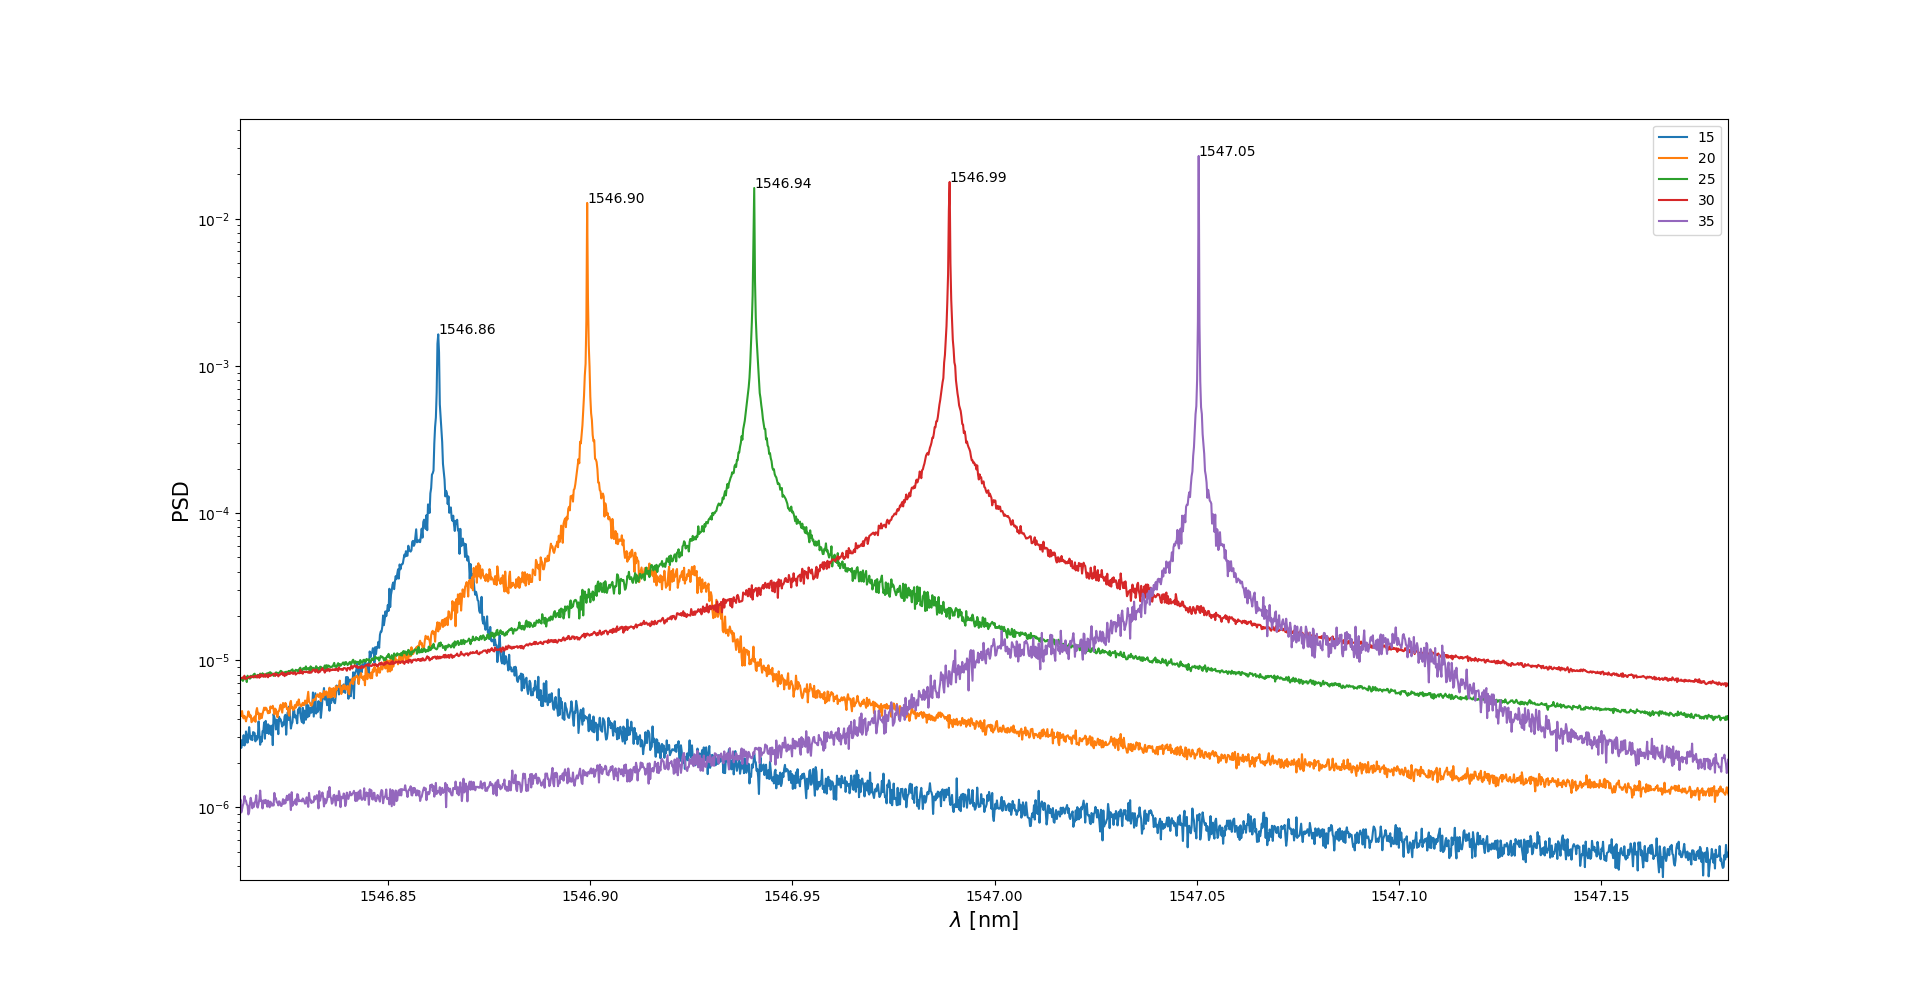
\includegraphics[width=1.0\linewidth, height=6cm]{Espectros.png}
				\caption{\label{Img:spectrosCW:sim}Espectros ópticos obtenidos mediante simulación.}
			\end{subfigure}
			\begin{subfigure}{0.45\textwidth}
				\centering
				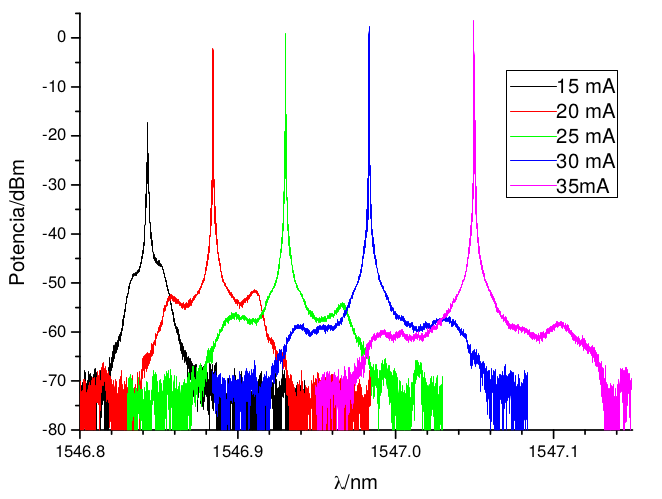
\includegraphics[width=1.0\linewidth, height=6cm]{../Chaves/OFC-GS/espectros_continua.png}
				\caption{\label{Img:spectrosCW:exp}Espectros ópticos obtenidos experimentalmente.}	
			\end{subfigure}
			\caption{\label{Img:spectrosCW}Espectros ópticos del DML para diferentes corrientes de polarización \ibias obtenidos mediante simulación (izquierda \ref{Img:spectrosCW:sim}) y mediante experimento (derecha, \ref{Img:spectrosCW:exp}).}
		\end{figure}

		Comparando los espectros obtenidos mediante simulación con los obtenidos esperimentalmente se observa un gran parecido en la forma, observando una forma m\'as puntiaguda y estrecha en los espectros con corriente $I_{Bias}= 15$ mA para ambas gr\'aficas. Adem\'as, la simulación permite observar los picos propios de las oscilaciones de relajaci\'on del l\'aser que se observan en el experimento.

		Adem\'as, a partir de los espectros de la Figura \ref{Img:spectrosCW} se pueden obtener las longitudes de onda de los picos de emisión en funci'on de la corriente \ibias. En la Tabla \ref{tab:lambdas} se muestran los valores de las longitudes de onda $lambda$ obtenidas de los espectros de la Figura \ref{Img:spectrosCW} tanto para la simulaci\'on como para el experimento.

		% tab:lambdas
		\begin{table}[H]
			\centering
			\begin{tabular}{c c c}
				\hline
				\ibias & $\lambda_{sim}$ & $\lambda_{exp}$ \\\hline 
				15 & 1546.86 & 1546.84 \\
				20 & 1546.90 & 1546.88 \\
				25 & 1546.94 & 1546.93 \\
				30 & 1546.99 & 1546.98 \\
				35 & 1547.05 & 1547.05 \\\hline
			\end{tabular}
			\caption{\label{tab:lambdas}Longitud de onda de las lineas de emisión del DML en función de la \ibias obtenidas de la figura \ref{Img:spectrosCW}. Se muestran los valores experimentales $\lambda_{exp}$ obtenidos de la gráfica \ref{Img:spectrosCW:exp} con un error de $\delta\lambda_{exp} = 0.02$, y los valores obtenidos de la simulación de la gráfica \ref{Img:spectrosCW:sim}.}
		\end{table}

	Los valores de las longitudes de onda que se muestran en la Tabla \ref{tab:lambdas} muestran una gran similitud entre los valores experimentales y los obtenidos mediante simulación, obteniendo una discrepancia m\'axima de $0.02$ nm. De esta forma, la gran concordancia entre los valores de $\lambda$ experimentales y los obtenidos a partir de la simulaci\'on, junto con la gran similitud en la forma de los espectros, muestra la capacidad de la simulaci\'on de reproducir computacionalmente los resultados obtenidos experimentalmente en el laboratorio.

	Para el estudio de la inyecci'on de luz se trabajar\'a con una corriente $I_{Bias} = 35$ mA. Por tanto, la Tabla \ref{tab:lambdas} permite obtener su longitud de onda de emisi\'on de $\lambda = 1547.05$ nm, siendo adem\'as la misma que la obtenida en el experimento.

\addtocontents{toc}{\vspace{0.1cm}}
\subsection{Oscilaciones de Relajaci\'on}

	Para que el l\'aser comience a emitir se ha de cumplir que la emisi\'on estimulada domine frente a la emisi\'on espont\'anea. Esto se produce cuando la densidad de portadores de carga en la regi\'on activa supera un valor umbral, $N_{th}$, a partir del cu\'al el l\'aser comienza a emitir fotones. Si la inyecci\'in de corriente que se le aplica al l\'aser es constante (\cw), la densidad de portadores de carga tender\'a a estabilizarse en $N_{th}$. De el mismo modo, la densidad de fotones y el chirp se estabilizar\'an para valores $S_{th}$ y $\Phi_{th}$.

	No obstante, si se parte de unas condiciones iniciales del l\'aser con valores $N(t=0) < N_{th}$, ser\'a necesario que transcurra un cierto tiempo hasta que el l\'aser alcance el equilibrio y se estabilice. A este tiempo se le denomina transitorio.

	Cabe destacar que, tal y como se coment\'o en el apartado \ref{Mdl:Code:Trans}, para la simulación se ha trabajado con un tiempo de transitorio $t_{trans} = 1.2$ ns, en el cu\'al se ha operado con la raiz cuadrada del m\'odulo de $S$ en los t\'erminos de ruido para evitar resultados complejos, despeciando dicho intervalo en el estudio de los espectros. Sin embargo, en este apartado se estudiar\'an las ecuaciones de balance en el transitorio para corrinte continua. El trabajar con una corriente continua mayor que la corriente umbral permite disminuir el intervalo de tiempo en el que se operar\'a con $\sqrt{|S|}$ hasta los 0.2 ns, pudiendo realizar un estudio m\'as riguroso de las ecuaciones de balance en el transitorio.

	Se considerar\'a una intensidad de corriente $I(t)$ funci\'on escal\'on con $I(t>0) = I_{Bias}$. En la ecuaci\'on \ref{eq:transient} se muestra la funci\'on escal\'on $I(t)$ utilizada as\'i como las condiciones iniciales para la densidad de portadores de carga $N(0)$, la densidad de fotones $S(0)$ y de la fase \'optica $\Phi(0)$.

		%eq:transient
		\begin{equation}
			\begin{matrix}
					I(t) = \left\{\begin{matrix}
									0 & t \leq 0\\ 
									I_{Bias} = 30 \textrm{mA} & t > 0
							\end{matrix}\right.
					& & & & & & 
					\begin{matrix}
						N(0) = N_{tr} \\ S(0) = 10^{15} \textrm{m}^{-3}\\ \Phi(0) = 0
					\end{matrix}
				\end{matrix}
			\label{eq:transient}
		\end{equation}

	En la Figura \ref{Img:transitorio} se muestra la evoluci\'on temporal de la \I\ junto con los valores obtenidos en la simulaci\'on para la \n\, la \s\ y la \fase\ para el transitorio $t_{trans} = 1.2$ ns.

		% Img:transitorio
		\begin{figure}[H]
			\centering
			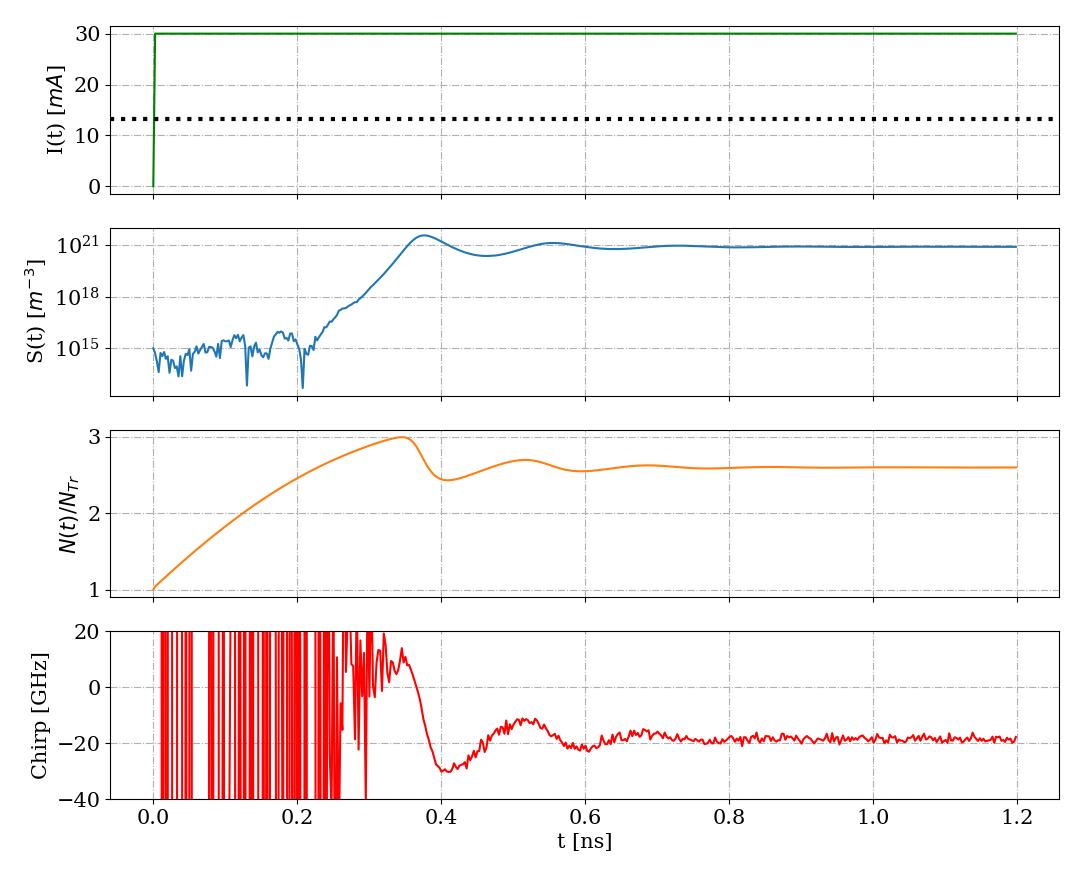
\includegraphics[width=0.7\linewidth]{transitorio.png}
			\caption{\label{Img:transitorio}Evoluci\'on temporal de la \I, la \s, la \n\ y del \chirp\ durante el transitorio. Para la \I\ se ha marcado la corriente umbral del l\'aser $I_{th} = 14.8$ mA con una l\'inea horizontal discontinua.}	
		\end{figure}
		
		Se observan en las evoluciones temporales de \n, \s\ y \fase\ de la Figura \ref{Img:transitorio} tres regiones diferentes en funci\'on del comportamiento de las tres magnitudes: $i$) Una vez que la corriente inyectada supera la corriente umbral $I_{th}$ (en $t=0$) la \n\ comienza a aumentar. No obstante, el valor de $N(t)$ se mantiene inferior a $N_{th}$ por lo que no se produce emisión estimulada, y as\'i, la densidad de fotones no aumenta y toma valores aleatorios, debido a la emisi\'on espont\'anea, alrededor de $S(0)$. Esto tambi\'en se puede observar en el comportamiento tambi\'en aleatorio del \chirp. $ii$) La \n\ continua aumentando alcanzando el valor umbral $N_{th}$ en $t = 0.23$ ns. En este punto la densidad de fotones comienza a aumentar debido a la emisi\'on estimulada producida al superar $N_{th}$. Sin embargo, al encontrarse $S(t)$ por debajo de $S_{th}$, $N(t)$ continua creciendo tomando valores por encima $N_{th}$ hasta que $S(t)$ alcanza el valor de $S_{th}$, en $t \approx 0.37$ ns. Al alcanzar $S(t)$ el valor de $S_{th}$, comienza a dominar la emisi\'on estimulada frente a la emisi\'on espont\'anea. Al alcanzar el valor $S_{th}$ la emisi\'on estimulada domina frente a la emisi\'on espont\'anea, como se puede observar el \chirp, y la densidad de portadores de carga comienza a disminuir, alcanzando la \n\ y \chirp\ un m\'aximo. La densidad de fotones contin\'ua aumentando y la densidad de portadores de carga disminuyendo, llegando nuevamente a tomar valores por debajo de $N_{th}$. Debido a \'esto $S(t)$ alcanza un m\'aximo cuando $N(t) = N_{th}$ y comienza a disminuir, volviendo a tomar valores inferiores a $S_{th}$ y as\'i, volviendo a aumentar $N(t)$. Estas oscilaciones entorno a los valores umbrales continuan, disminuyendo su amplitud, realizando un comportamiento anarm\'onico y se las conoce como oscilaciones de relajaci\'on. En la figura \ref{Img:transitorio} se observan claramente estas oscilaciones, siendo iguales en el tiempo para \n\ y para el \chirp\ (m\'aximos en el mismo tiempo $t$). Tambi\'en se observa la relaci\'on entre las oscilaciones de \'estas magnitudes con las de $S(t)$, obteniendo un m\'aximo en $S(t)$ cuando $N(t) = N_{th}$ de tal forma que ambas oscilaciones tengan el mismo periodo. $ii$) Las oscilaciones de relajaci\'on van disminuyendo a medida que el tiempo avanza alcanzando el equilibrio en el que las tres magnitudes se mantienen constante.

		A partir de los datos de la figura \ref{Img:transitorio} se pueden obtener las frecuencias de las oscilaciones de relajaci\'on en el transitorio, a patir del tiempo entre los m\'aximos. Una primera estimaci\'on permite obtener una frecuencia de oscilaci\'on de $\nu_{RoF} \approx 5.9$ GHz, que pasado a longitud de onda equivale a $\lambda = 0.05$ nm. Comparando dicho valor con los picos debidos a las oscilaciones de relajaci\'on de los espectros para $I = 30$ mA de la figura \ref{Img:spectrosCW} observamos que se encuentran en el mismo orden de magnitud, mostrando una gran concordancia entre la simulaci\'on y el experimento.
